\chapter{Anhang}
\thispagestyle{fancy}

Dies ist ein Beispiel für einen \gls{Glossareintrag}.

\begin{figure}[h]
\centering

\includegraphics[scale=0.5]{pics/Beispiel.png}
\caption{Das ist ein Beispielbild.}
\end{figure}

\lipsum[1-3]

\begin{figure}[htbp]
	
	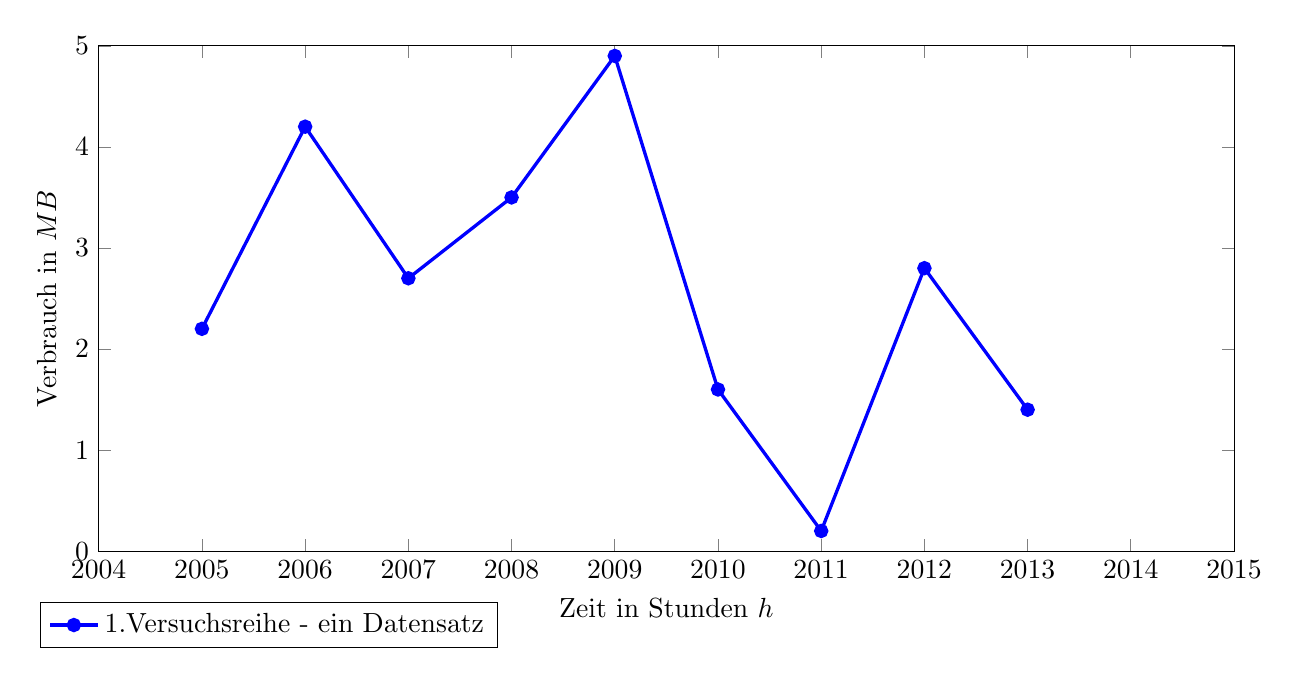
\begin{tikzpicture} 
	\title{}
	\begin{axis}[ x tick label style={/pgf/number format/1000 sep=},
	%xtick=data,
	xmin=2004,
	xmax=2015,
	ymin=0,
	ymax=5,
	width=16cm,
	height=8cm,
	ylabel={Verbrauch in $MB$},
	xlabel={Zeit in Stunden $h$}
	]
	\pgfplotsset{every axis legend/.append style={
			at={(0.15,-0.1)},
			anchor=north}}
		\addplot[very thick,color=blue, mark=*] table[x=year, y=value, ignore chars=*] {
			year	value
			2013    1.40
			2012    2.80
			2011    0.20
			2010    1.60
			2009    4.90
			2008    3.50
			2007    2.70
			2006    4.20
			2005    2.20

		};
	\addlegendentry{1.Versuchsreihe - ein Datensatz}
	\end{axis} 
	\end{tikzpicture}
	\caption{Datenverbrauch pro Stunde}
\end{figure}